% !TEX program = pdflatex
\documentclass[12pt]{article}
 \usepackage[margin=1in]{geometry} 
\usepackage{amsmath,amsthm,amssymb,amsfonts, enumitem, fancyhdr, color, comment, graphicx, environ}
\pagestyle{fancy}
\setlength{\headheight}{65pt}
\newenvironment{problem}[2][Problem]{\begin{trivlist}
\item[\hskip \labelsep {\bfseries #1}\hskip \labelsep {\bfseries #2.}]}{\end{trivlist}}
\newenvironment{sol}
    {\emph{Solution:}
    }
    {
    \qed
    }
\specialcomment{com}{ \color{blue} \textbf{Comment:} }{\color{black}}
\NewEnviron{probscore}{\marginpar{ \color{blue} \tiny Problem Score: \BODY \color{black} }}
\usepackage[UTF8]{ctex}
\usepackage[version=4]{mhchem}
\lhead{Name: 陈稼霖\\ StudentID: 45875852}
\rhead{CHEM1111 \\ General Chemistry II \\ Spring 2019 \\ Homework 3}
\begin{document}
\begin{problem}{15.29}
(a) Calculate the pH of a $0.20$ \textsc{m} solution of benzoic acid at $25 ^{\circ}$C.\\
(b) How many moles of acetic acid must be dissolved per liter of water to obtain the same pH as that from part (a)?
\end{problem}
\begin{sol}
\\(a) Suppose the change of concentration of benzoic acid is $-x$ \textsc{m}, then
\begin{table}[h]
\centering
\begin{tabular}{cccccccc}
& \ce{C6H5COOH(aq)} & + & \ce{H2O(l)} & \ce{<=>} & \ce{H3O+(aq)} & \ce{+} & \ce{C6H5COO-(aq)} \\
Initial, \textsc{m} & $0.20$ & & & & $0$ & & $0$ \\
Change, \textsc{m} & $-x$ & & & & $x$ & & $x$ \\
Equilibrium, \textsc{m} & $0.20-x$ & & & & $x$ & & $x$
\end{tabular}
\end{table}
\\The ionization constant of benzoic acid is $K_a=6.46\times10^{-5}$, so
\[
K_a=\frac{[H_3O^+][C_6H_5COO^-]}{[C_6H_5COOH]}=\frac{x^2}{0.20-x}=6.46\times10^{-5}
\]
Because the ionization constant of benzoic acid, $K_a$ is very small, the change of the concentration of \ce{C_6H_5COOH}, $-x$, is much smaller than its initial concentration. In this way, we have the following approximation
\[
K_a=6.46\times10^{-5}\approx\frac{x^2}{0.20}\Longrightarrow x=3.6\times10^{-3}mol\cdot L^{-1}
\]
So the equilibrium concentration of \ce{H3O+} is
\[
[H_3O^+]=xmol\cdot L^{-1}=3.6\times10^{-3}mol\cdot L^{-1}
\]
Therefore, the $pH$ of the benzoic acid solution is
\[
pH=-\log_{10}[H_3O^+]=-\log_{10}(3.6\times10^{-3})=\uline{2.44}
\]
(b) To obtain the same pH as that form part (a), the concentration of \ce{H_3O^+} need to be $3.6\times10^{-3}mol\cdot L^{-1}$.\\
Suppose $n$ mol acetic acid is dissolved per liter of water, then
\begin{table}[h]
\centering
\begin{tabular}{cccccccc}
& \ce{CH3COOH(aq)} & + & \ce{H2O(l)} & \ce{<=>} & \ce{H3O+(aq)} & \ce{+} & \ce{CH3COO-(aq)} \\
Initial, \textsc{m} & $n$ & & & & $0$ & & $0$ \\
Change, \textsc{m} & $-3.6\times10^{-3}$ & & & & $3.6\times10^{-3}$ & & $3.6\times10^{-3}$ \\
Equilibrium, \textsc{m} & $n-3.6\times10^{-3}$ & & & & $3.6\times10^{-3}$ & & $3.6\times10^{-3}$
\end{tabular}
\end{table}
\\The ionization constant of acetic acid is $K_a=1.76\times10^{-5}$, so
\[
K_a=\frac{[H_3O^+][CH_3COO^-]}{[CH_3COOH]}=\frac{(3.6\times10^{-3})^2}{n-3.6\times10^{-3}}=1.76\times10^{-5}\Longrightarrow n=0.74
\]
Therefore, \uline{$0.74$ mol} of acetic acid must be dissolved per liter of water.
\end{sol}

\begin{problem}{15.42}
Suppose a $0.100$ \textsc{m} solution of each of the following substances is prepared. Rank the pH of the resulting solutions from lowest to highest: \ce{KF}, \ce{NH4I}, \ce{HBr}, \ce{NaCl}, \ce{LiOH}.
\end{problem}
\begin{sol}
\ce{KF} is a salt of the weak acid \ce{HF} and the strong base \ce{KOH}, so the pH of its solution is little more than $7$.\\
\ce{NH4I} is a salt of the strong acid \ce{HI} and the weak base \ce{NH3}, so the pH of its solution is little less than $7$.\\
\ce{HBr} is a strong acid, so the pH of its solution is much less than $7$.\\
\ce{NaCl} is a salt of the strong acid \ce{HCl} and strong base \ce{NaOH}, so the pH of its solution is $7$.\\
\ce{LiOH} is a strong base, so the pH of its solution is much more than $7$.\\
Therefore, rank of the resulting solution's pH from lowest to highest is:
\begin{center}
\uline{pH(\ce{HBr})$<$pH(\ce{NH4I})$<$pH(\ce{NaCl})$<$pH(\ce{KF})$<$pH(\ce{LiOH})}.
\end{center}
\end{sol}

\begin{problem}{15.43}
“Tris” is short for tris(hydroxymethyl)aminomethane. This weak base is widely used in biochemical research for the preparation of buffers. It offers low toxicity and a p$K_b$ ($5.92$ at $25 ^{\circ}$C) that is convenient for the control of pH in clinical applications. A buffer is prepared by mixing $0.050$ mol of tris with 0.025 mol of \ce{HCl} in a volume of $2.00$ L. Compute the pH of the solution.
\end{problem}
\begin{sol}
The $pK_a$ of the conjugate acid of tris, \ce{(CH2OH)3CNH3^+}, is
\[
pK_a=14-pK_b=14-5.92=8.08
\]
The reaction equation of tris with \ce{HCl} is
\begin{center}
\ce{(CH2OH)3CNH2 + H^+ ->(CH2OH)3CNH3^+}
\end{center}
After mixing $0.050$ mol of tris with $0.025$ mol of \ce{HCl}, the initial number of moles of tris and \ce{(CH_2OH)_3CNH_3^+} are
\[
n((CH_2OH)_3CNH_2)=0.025mol,~~n((CH_2OH)_3CNH_3^+)=0.025mol
\]
so their initial concentration after mixing are
\begin{gather*}
[(CH_2OH)_3CNH_2]=\frac{n((CH_2OH)_3CNH_2)}{V}=\frac{0.025mol}{2L}=0.0125mol\cdot L^{-1}\\
[(CH_2OH)_3CNH_3^+]=\frac{n((CH_2OH)_3CNH_3^+)}{V}=\frac{0.025mol}{2L}=0.0125mol\cdot L^{-1}
\end{gather*}
Therefore, the pH of the solution is
\[
pH=pK_a-\log_{10}\frac{[(CH_2OH)_3CNH_3^+]_0}{[(CH_2OH)_3CNH_2]_0}=8.08-\log_{10}\frac{0.0125mol\cdot L^{-1}}{0.0125mol\cdot L^{-1}}=\uline{8.08}
\]
\end{sol}

\begin{problem}{15.49}
You have at your disposal an ample quantity of a solution of $0.0500$ \textsc{m} \ce{NaOH} and $500$ mL of a solution of \ce{0.100} \textsc{m} formic acid (\ce{HCOOH}). How much of the \ce{NaOH} solution should be added to the acid solution to produce a buffer of pH $4.00$?
\end{problem}
\begin{sol}
The ionization constant of \ce{HCOOH} is $pK_a=1.77\times10^{-4}$. The pH of the buffer is
\[
4.00=pH=pK_a-\log_{10}\frac{[HCOOH]}{[HCOO^-]}=-\log_{10}(1.77\times10^{-4})-\log_{10}\frac{[HCOOH]}{[HCOO^-]}
\]
so the ratio of the initial concentration of \ce{HCOOH} and \ce{HCOO-} after reaction should be
\[
\frac{[HCOOH]}{[HCOO^-]}=0.565
\]
The initial number of moles of \ce{HCOOH} is
\[
n_0(HCOOH)=c_0(HCOOH)V_0=0.100mol\cdot L^{-1}\times0.500L=0.0500mol
\]
Suppose the volume of the \ce{NaOH} solution added is $V(NaOH)$ and the volume of the buffer solution is $V$ after the reaction is $V$, the ratio of the initial concentration of \ce{HCOOH} and \ce{HCOO-} after reaction is
\begin{gather*}
\begin{align*}
\frac{[HCOOH]}{[HCOO^-]}=&\frac{\frac{n_0(HCOOH)-c(NaOH)V(NaOH)}{V}}{\frac{c(NaOH)V(NaOH)}{V}}\\
=&\frac{n_0(HCOOH)-c(NaOH)V(NaOH)}{c(NaOH)V(NaOH)}\\
=&\frac{0.0500mol-0.0500mol\cdot L^{-1}\times V(NaOH)}{0.0500mol\cdot L^{-1}\times V(NaOH)}=0.565
\end{align*}\\
\Longrightarrow V(NaOH)=0.639L=639mL
\end{gather*}
Therefore, \uline{$639$ mol} of the \ce{NaOH} solution should be added to the acid solution to produce a buffer of pH $4.00$.
\end{sol}

\begin{problem}{15.56}
Ammonia is a weak base with a $K_b$ of $1.8\times10^{-5}$. A $140.0$ mL sample of a $0.175$ \textsc{m} solution of aqueous ammonia is titrated with a $0.106$ \textsc{m} solution of the strong acid \ce{HCl}. The reaction is
\begin{center}
\ce{NH3(aq) + HCl(aq) ->NH4^+(aq) + Cl^-(aq)}
\end{center}
Compute the pH of the titration solution before any acid is added, when the titration is at the half-equivalence point, when the titration is at the equivalence point, and when the titration is $1.00$ mL past the equivalence point.
\end{problem}
\begin{sol}
The number of moles of the ammonia before titration is
\[
n_0(NH_3)=c_0(NH_3)V_0(NH_3)=0.175mol\cdot L^{-1}\times0.1400L=0.0245mol
\]
and the ionization constant of its conjugate acid, \ce{NH3} is
\[
K_a=\frac{K_w}{K_b}=\frac{10^{-14}}{1.8\times10^{-5}}=5.6\times10^{-10}
\]
\uline{Before any acid is added}: suppose the change of the concentration of ammonia is $-x$ \textsc{m}, then
\begin{table}[h]
\centering
\begin{tabular}{cccccccc}
& \ce{NH3(aq)} & + & \ce{H2O(l)} & \ce{<=>} & \ce{OH-(aq)} & \ce{+} & \ce{NH4^+(aq)} \\
Initial, \textsc{m} & $0.175$ & & & & $0$ & & $0$ \\
Change, \textsc{m} & $-x$ & & & & $x$ & & $x$ \\
Equilibrium, \textsc{m} & $0.175-x$ & & & & $x$ & & $x$
\end{tabular}
\end{table}
\\The ionization of ammonia is
\[
K_b=\frac{[OH^-][NH_4^+]}{NH_3}=\frac{x^2}{0.175-x}=1.8\times10^{-5}
\]
Because the ionization constant of ammonia, $K_b$, is very small, the change of the concentration of \ce{NH3}, $-x$, is much smaller than its initial concentration. In this way, we have the following approximation
\[
K_b=1.8\times10^{-5}\approx\frac{x^2}{0.175}\Longrightarrow x=1.77\times10^{-3}
\]
So the equilibrium concentration of \ce{OH-} is
\[
[OH^-]=xmol\cdot L^{-1}=1.77\times10^{-3}mol\cdot L^{-1}
\]
Therefore, the pH of the titration solution before any acid is added is
\[
pH=-\log_{10}[H^+]=-\log_{10}\frac{K_w}{[OH^-]}=-\log_{10}\frac{10^{-14}}{1.77\times10^{-3}}=\uline{11.25}
\]
\uline{When the titration is at the half}: the ratio of the \ce{NH4^+} and its conjugate, \ce{NH3} is $1$, so the pH of the titration solution is
\[
pH=pK_a-\log_{10}\frac{[NH_4^+]}{[NH_3]}=-\log_{10}5.5\times10^{-10}-\log_{10}1=\uline{9.26}
\]
\uline{When the titration is at the equivalence point}: the volume of \ce{HCl} solution added is
\[
V_{eq}(HCl)=\frac{n(NH_3)}{c_0(HCl)}=\frac{0.0245mol}{0.106mol\cdot L^{-1}}=0.231L
\]
Suppose the volume of the titration solution at the equivalence point is the sum of the initial volume of the ammonia solution and the volume of the \ce{HCl} solution added
\[
V_{eq}=V_0(NH_3)+V_{eq}(HCl)=0.1400L+0.231L=0.371L
\]
At the equivalence point, the initial concentration of \ce{NH4^+} is
\[
c_{eq}(NH_4^+)=\frac{n_eq(NH_4^+)}{V_{eq}}=\frac{n_0(NH_3)}{V_{eq}}=\frac{0.0245mol}{0.371L}=0.0660mol\cdot L^{-1}
\]
suppose the change of the concentration of \ce{NH4^+} is $-y$ \textsc{m}, then
\begin{table}[h]
\centering
\begin{tabular}{cccccccc}
& \ce{NH4^+(aq)} & + & \ce{H2O(l)} & \ce{<=>} & \ce{H+(aq)} & \ce{+} & \ce{NH3.H2O(aq)} \\
Initial, \textsc{m} & $0.0660$ & & & & $0$ & & $0$ \\
Change, \textsc{m} & $-y$ & & & & $y$ & & $y$ \\
Equilibrium, \textsc{m} & $0.0660-y$ & & & & $y$ & & $y$
\end{tabular}
\end{table}
\\The ionization constant of \ce{NH4^+} is
\[
K_a=\frac{[H^+][NH_3\cdot H_2O]}{[NH_4^+]}=\frac{y^2}{0.0660-y}=5.6\times10^{-10}
\]
Because the ionization constant of \ce{NH4^+}, $K_a$, is very small, the change of the concentration of \ce{NH4^+}, $-y$, is much smaller than its initial concentration. In this way, we have the following approximation
\[
K_a=5.6\times10^{-10}\approx\frac{y^2}{0.0660}\Longrightarrow y=6.08\times10^{-6}mol
\]
So the equilibrium concentration of \ce{H+} is
\[
[H^+]=ymol=6.08\times10^{-6}mol
\]
Therefore, the pH of the titration solution at the equivalence point is
\[
pH=-\log_{10}[H^+]=-\log_{10}(6.08\times10^{-6})=\uline{5.22}
\]
\uline{When the titration is $1.00$ mL past the equivalence point}: The volume of the \ce{HCl} solution added is
\[
V_1(HCl)=V_{eq}(HCl)+1.00\times10^{-3}L=0.232mL
\]
The volume of the titration solution is
\[
V_1=V_0(NH_3)+V_1(HCl)=0.1400L+0.232L=0.372L
\]
So the concentration of \ce{H^+} is approximately
\[
c_1(H^+)\approx\frac{c_0(HCl)\times1.00\times10^{-3}L}{V_1}=\frac{0.106mol\cdot L^{-1}\times1.00\times10^{-3}L}{0.372L}=2.85\times10^{-4}mol\cdot L^{-1}
\]
Therefore, the pH of the titration solution when the titration is $1.00$ mL past the equivalence point is
\[
pH=-\log_{10}[H^+]=-\log_{10}(2.85\times10^{-4})=\uline{3.55}
\]
\end{sol}

\begin{problem}{15.58}
An antacid tablet (such as Tums or Rolaids) weighs $1.3259$ g. The only acid-neutralizing ingredient in this brand of antacid is \ce{CaCO3} . When placed in $12.07$ mL of $1.070$ \textsc{m} \ce{HCl}, the tablet fizzes merrily as \ce{CO2}(g) is given off. After all of the \ce{CO2} has left the solution, an indicator is added, followed by $11.74$ mL of $0.5310$ \textsc{m} \ce{NaOH}. The indicator shows that at this point the solution is definitely basic. Addition of $5.12$ mL of $1.070$ \textsc{m} \ce{HCl} makes the solution acidic again. Then $3.17$ mL of the $0.5310$ \textsc{m} \ce{NaOH} brings the titration exactly to an endpoint, as signaled by the indicator. Compute the percentage by mass of \ce{CaCO3} in the tablet.
\end{problem}
\begin{sol}
The total number of moles of \ce{HCl} added is
\begin{align*}
n(HCl)=&c(HCl)(V_1(HCl)+V_2(HCl))=1.070mol\cdot L^{-1}\times(0.01207L+0.00512L)\\
=&0.01839mol
\end{align*}
The total number of moles of \ce{NaOH} added is
\begin{align*}
n(NaOH)=&c(NaOH)(V_1(NaOH)+V_2(NaOH))\\
=&0.5310mol\cdot L^{-1}\times(0.01174L+0.00317L)=7.917\times10^{-3}mol
\end{align*}
So the number of moles of \ce{CaCO3} in the tablet is
\[
n(CaCO_3)=\frac{n(HCl)-n(NaOH)}{2}=\frac{0.01839mol-7.917\times10^{-3}mol}{2}=0.0052365mol
\]
Therefore, the mass percentage of \ce{CaCO3} in the tablet is
\begin{align*}
\alpha(CaCO_3)=&\frac{n(CaCO_3)M(CaCO_3)}{m(tablet)}\times100\%=\frac{0.0052365mol\times100.1g\cdot mol^{-1}}{1.3259g}\times100\%\\
=&\uline{39.53\%}
\end{align*}
\end{sol}

\begin{problem}{15.66}
Oxalic acid ionizes in two stages in aqueous solution:
\begin{center}
\ce{H2C2O4(aq) + H2O(l) <=>H3O+(aq) + HC2O4-(aq)}, $K_{a1}=5.9\times10^{-2}$\\
\ce{HC2O4^-(aq) + H2O(l) <=>H3O+(aq) + C2O4^{2-}(aq)}, $K_{a2}=6.4\times10^{-5}$
\end{center}
Calculate the equilibrium concentrations of \ce{C2O4^{2-}}, \ce{HC2O4^-}, \ce{H2C2O4}, and \ce{OH-} in a $0.10$ \textsc{m} solution of sodium oxalate (\ce{Na2C2O4}).
\end{problem}
\begin{sol}
Sodium oxalate is a salt of weak acid and strong weak, so we assume it hydrolyzes completely at first and then ionizes a little. The equation of hydrolyzation is
\begin{center}
\ce{C2O4^{2-}(aq) + 2H2O(l) ->2OH-(aq) + H2C2O4(aq)}
\end{center}
So the concentration of \ce{OH-} is
\[
\uline{[OH^-]}=c_0(Na_2C_2O_4)=2\times0.10mol\cdot L^{-1}=\uline{0.20mol\cdot L^{-1}}
\]
Suppose the change of the concentration of \ce{H2C2O4} at first step of ionization is $-x$ \textsc{m}, then
\begin{table}[h]
\centering
\begin{tabular}{cccccccc}
& \ce{H2C2O4(aq)} & + & \ce{H2O(l)} & \ce{<=>} & \ce{H3O+(aq)} & \ce{+} & \ce{HC2O4^-(aq)} \\
Initial, \textsc{m} & $0.10$ & & & & $0$ & & $0$ \\
Change, \textsc{m} & $-x$ & & & & $x$ & & $x$ \\
Equilibrium, \textsc{m} & $0.10-x$ & & & & $x$ & & $x$
\end{tabular}
\end{table}
\\The ionization constant of the first step of ionization is
\begin{gather*}
K_{a2}=\frac{[H^+][HC_2O_4^-]}{[H_2C_2O_4]}=\frac{x^2}{0.10-x}=5.9\times10^{-2}\\
\Longrightarrow x=0.53\text{ or }-0.11\text{ (unphysical!)}
\end{gather*}
So the concentration of \ce{H2C2O4} is
\[
\uline{[H_2C_2O_4]}=0.10mol\cdot L^{-1}-xmol\cdot L^{-1}=0.10mol\cdot L^{-1}-0.53mol\cdot L^{-1}=\uline{0.047mol\cdot L^{-1}}
\]
and the concentration of \ce{HC2O4^-} and \ce{H+} after the first step of ionization is
\[
\uline{[HC_2O_4^-]}=[H+]_1=xmol\cdot L^{-1}=\uline{0.053mol\cdot L^{-1}}\\
\]
Suppose the change of the concentration of \ce{HC2O4^-} is $-y$ \textsc{m}, then
\begin{table}[h]
\centering
\begin{tabular}{cccccccc}
& \ce{HC2O4^-(aq)} & + & \ce{H2O(l)} & \ce{<=>} & \ce{H3O+(aq)} & \ce{+} & \ce{C2O4^{2-}(aq)} \\
Initial, \textsc{m} & $0.047$ & & & & $0.053$ & & $0$ \\
Change, \textsc{m} & $-y$ & & & & $y$ & & $y$ \\
Equilibrium, \textsc{m} & $0.047-y$ & & & & $0.053+y$ & & $y$
\end{tabular}
\end{table}
The ionization constant of the second step of the ionization is
\[
K_{a2}=\frac{[H_3O^+][C_2O_4^{2-}]}{[HC_2O_4^-]}=\frac{(0.053+y)y}{0.047-y}=6.4\times10^{-5}mol\cdot L^{-1}
\]
Because the ionization constant, $K_{a2}$, is very small, the change of the concentration of \ce{HC2O4^-}, $y$, is much smaller than $[HC_2O_4^-]$ and $[H+]_1$. In this way, we have the following approximation
\[
K_{a2}=6.4\times10^{-5}mol\cdot L^{-1}=\frac{0.053x}{0.047}\Longrightarrow y=5.7\times10^{-5}mol\cdot L^{-1}
\]
So the concentration of \ce{C2O4^{2-}} is
\[
\uline{[C_2O_4^{2-}]}=ymol=\uline{6.4\times10^{-5}mol\cdot L^{-1}}
\]
Therefore,
\begin{align*}
[C_2O_4^{2-}]=&6.4\times10^{-5}mol\cdot L^{-1}\\
[HC_2O_4^-]=&0.053mol\cdot L^{-1}\\
[H_2C_2O_4]=&0.047mol\cdot L^{-1}\\
[OH^-]=&0.20mol\cdot L^{-1}
\end{align*}
\end{sol}

\begin{problem}{15.73}
Which will be the stronger acid: benzene (\ce{C6H6}) or cyclohexane (\ce{C6H12})? Explain by using resonance Lewis structures.
\end{problem}
\begin{sol}
We can write only one Lewis diagram for the conjugate base of cyclohexane as shown in Figure \ref{1}.
\begin{figure}[h]
\centering
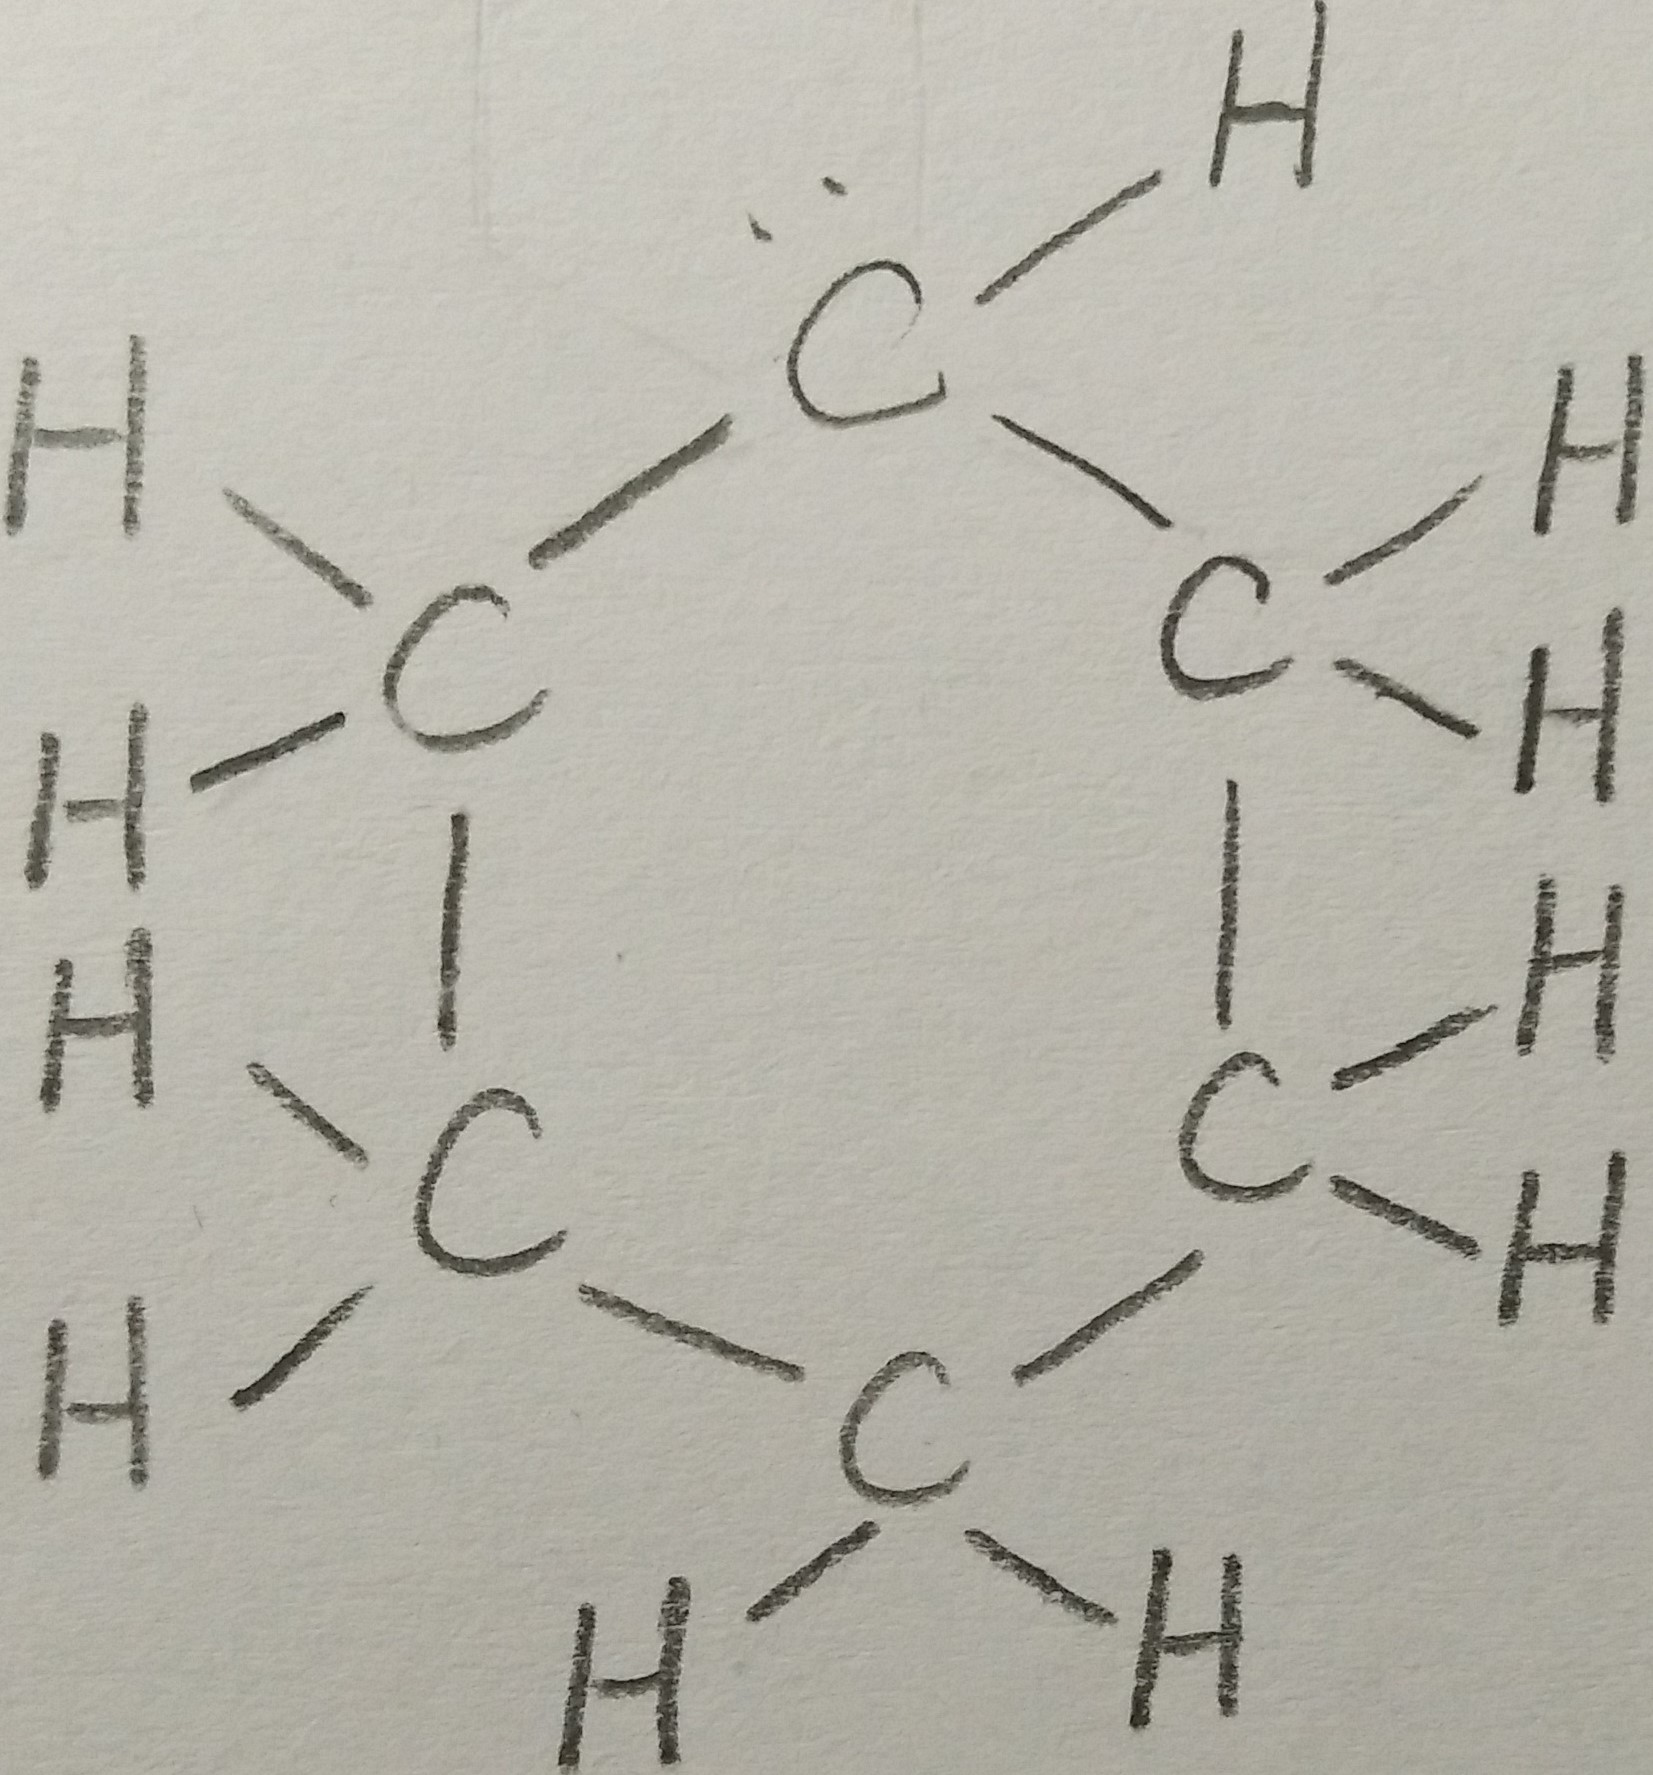
\includegraphics[scale=.1]{15_73_1.jpg}
\caption{Problem 15.73 Lewis diagram for the conjugate base of cyclohexane}\label{1}
\end{figure}
\\while we can write two resonance diagrams for the conjugate
base of benzene as shown in Figure \ref{2} which is very stable.
\begin{figure}[h]
\centering
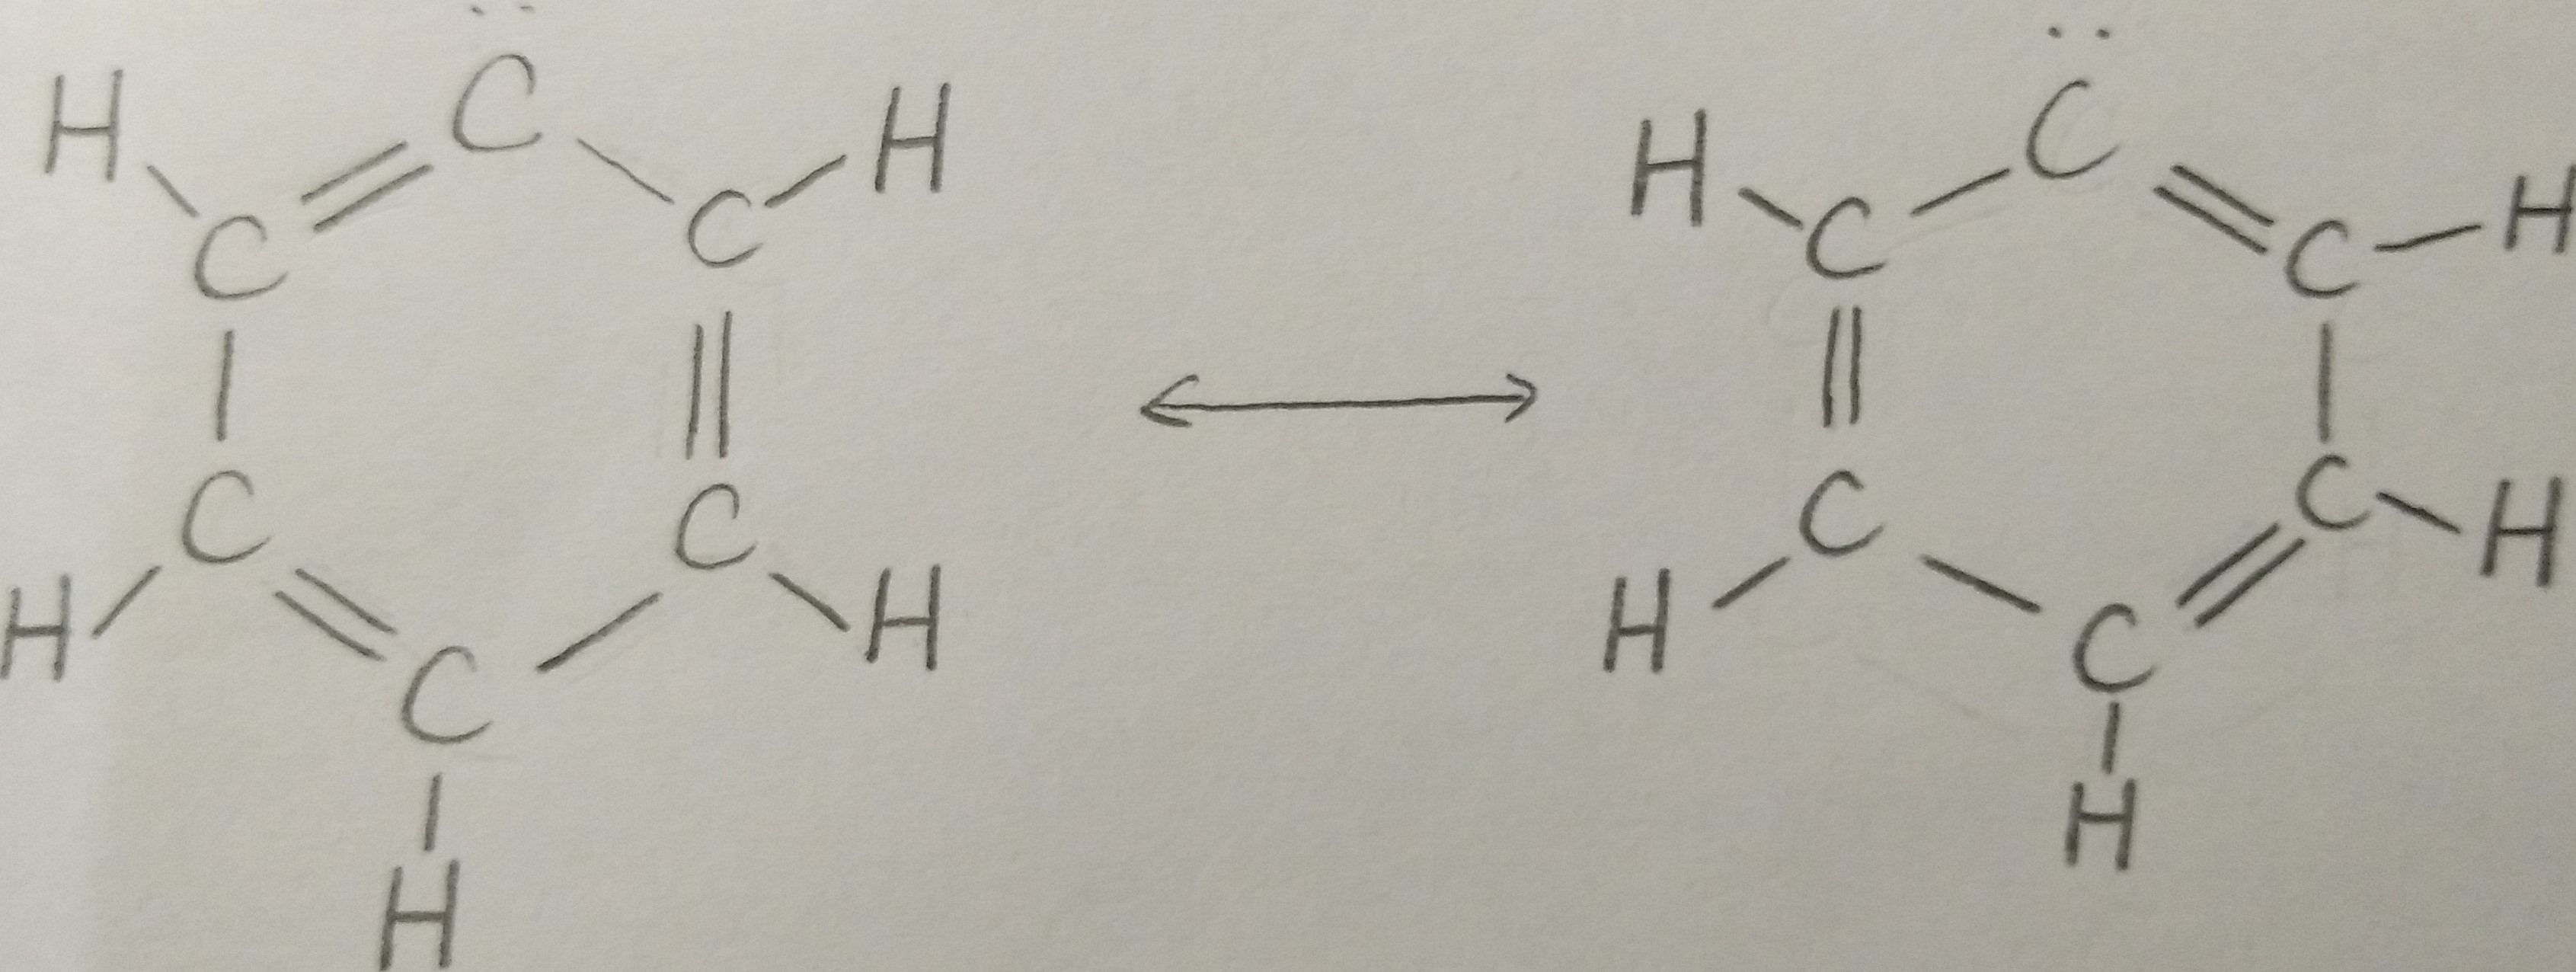
\includegraphics[scale=.1]{15_73_2.jpg}
\caption{Problem 15.73 Resonance diagrams for the conjugate
base of benzene}\label{2}
\end{figure}
Therefore, \uline{\ce{C6H6} is the stronger acid}.
\end{sol}

\begin{problem}{15.75}
For each of the following pairs of molecules, predict which is the stronger acid.\\
(a) \ce{CF3COOH} or \ce{CCl3COOH}\\
(b) \ce{CH2FCH2CH2COOH} or \ce{CH3CH2CHFCOOH}\\
(c) \ce{(C6H5)COOH} or \ce{(C(CH3)3)2(C6H5)COOH}
\end{problem}
\begin{sol}
(a) \uline{\ce{CF3COOH} is the stronger acid}, because atoms \ce{F} are more electronegative than atoms \ce{Cl} and, therefore, have stronger attraction on the electrons in the carboxyl to make it easier for the atom \ce{H} in the carboxyl to ionize.\\
(b) \uline{\ce{CH3CH2CHFCOOH} is the stronger acid}, becuae atom \ce{F} in \ce{CH3CH2CHFCOOH} is closer to the atom \ce{H} in the carboxyl than it in \ce{CH2FCH2CH2COOH} and, therefore have stronger attraction on the electrons in the carboxyl to make it easier for the atom \ce{H} in the carboxyl to ionize.\\
(c) \uline{\ce{(C6H5)COOH} is the stronger acid}, because the accessory groups on the second one have repulsion on the electrons in the carboxyl to make the atom \ce{H} in the carboxyl not so easy to ionize.
\end{sol}

\begin{problem}{15.78}
A sample of vinegar contains $40.0$ g of acetic acid (\ce{CH3COOH}) per liter of solution. Suppose $1.00$ mL is removed and diluted to $1.00$ L, and $1.00$ mL of that solution is removed and diluted to $1.00$ L. Calculate the pH of the resulting solution. (Hint: This is a sufficiently dilute solution that the autoionization of water cannot be neglected.)
\end{problem}
\begin{sol}
The concentration of acetic acid in the original solution is
\[
c_1(CH_3COOH)=\frac{m(CH_3COOH)/M(CH_3COOH)}{V_0}=\frac{40.0g/60.1g\cdot mol^{-1}}{1L}=0.666mol
\]
The concentration of diluted acetic acid is
\[
c_2(CH_3COOH)=\frac{c_1(CH_3COOH)V_1}{V_2}\times\frac{V_3}{V_4}=\frac{0.666mol\cdot L^{-1}\times0.00100mL}{1.00L}\times\frac{0.00100mL}{1.00L}=6.66\times10^{-7}mol\cdot L^{-1}
\]
Suppose the change of concentration of \ce{CH_3COOH} during ionization is $-x$ \textsc{m}, then
\begin{table}[h]
\centering
\begin{tabular}{cccccccc}
& \ce{CH3COOH(aq)} & + & \ce{H2O(l)} & \ce{<=>} & \ce{H3O+(aq)} & \ce{+} & \ce{CH3COO^-(aq)} \\
Initial, \textsc{m} & $6.66\times10^{-7}$ & & & & $10^{-7}$ & & $0$ \\
Change, \textsc{m} & $-x$ & & & & $x$ & & $x$ \\
Equilibrium, \textsc{m} & $6.66\times10^{-7}-x$ & & & & $10^{-7}+x$ & & $x$
\end{tabular}
\end{table}
The ionization constant of \ce{CH3COOH} is
\begin{gather*}
K_a=\frac{[H_3O^+][CH_3COO^-]}{[CH_3COOH]}=\frac{(10^{-7}+x)x}{6.66\times10^{-7}-x}=1.76\times10^{-5}\\
\Longrightarrow x=6.39\times10^{-7}\text{ or }-1.83\times10^{-5}\text{ (unphysical!)}
\end{gather*}
So the concentration of \ce{H+} in the resulting solution is
\[
[H^+]=10^{-7}mol\cdot L^{-1}+xmol\cdot L^{-1}=10^{-7}mol\cdot L^{-1}+6.39\times10^{-7}mol\cdot L^{-1}=7.39\times10^{-7}mol\cdot L^{-1}
\]
Therefore, the pH of the resulting solution is
\[
pH=-\log_{10}[H^+]=-\log_{10}(7.39\times10^{-7})=\uline{6.13}
\]
\end{sol}
\end{document}